\subsubsection{Non-linear Hypothesis}
\begin{itemize}[--]
	\item Suppose you have a housing classification problem with different features $x_1, \ldots ,x_100$ and if we were to include all quadratic terms for linear classification there would be an enourmous number of terms (~5000 features).
	\item Using linear classifiers has an extremely bad asymptotic complexity (n is typically large)
	\item For example computer vision problems are $\O{n^2}$
	\item Neural networks turn out to be a much better way to solve these style problems
\end{itemize}

\subsubsection{Neurons and the Brain}
\begin{itemize}[--]
	\item Neural networks origins are in algorithms that try to mimic the brain
	\item \textbf{``One learning algorithm hypothesis''}: $x$ cortex can learn whatever is hooked up to it
	\begin{itemize}[--]
		\item Auditory cortex can learn to see
		\item Somatosensory cortex (touch) can learn to see
		\item There is one algorithm that can teach anything to do any function
	\end{itemize}
\end{itemize}

\subsubsection{Model Representation I}
\begin{itemize}[--]
	\item Neural networks work by simulating the neurons in the brain
	\item Has ``input wires'' dendrite
	\item Has ``output wires'' axon
	\item Neuron is a computational unit that takes in inputs and produces an output
	\item Neurons communicate with little spikes of electricity through their axons, which another neuron can receiv with its dendrite
	\item In an artificial neural network we model a neuron as a logistic unit:
	\begin{center}\begin{tikzpicture}[node distance=1cm, auto]
		%Place nodes
		\node (x1) {$x_1$};
		\node [below of=x1] (dots) {$x_2$};
		\node [below of=dots] (xn) {$x_3$};

		\node [cloud, right of=dots] (neuron) {  };

		\node [right of=neuron] (h) {$h_\theta (x)$};

		%Draw edges
		\path [line] (x1) -- (neuron);
		\path [line] (dots) -- (neuron);
		\path [line] (xn) -- (neuron);
		\path [line] (neuron) -- (h);
	\end{tikzpicture}\end{center}

		$$x=\begin{bmatrix} x_0\\ x_1\\ x_2\\ x_3 \end{bmatrix}, \theta=\begin{bmatrix}\theta_0 \\ \theta_1 \\ \theta_2 \\ \theta_3 \end{bmatrix}, h(x)=\frac{1}{1+e^{-\theta^{T}x}}$$

	\begin{itemize}[--]
		\item Here the arrows coming from the $x$ are the input wires
		\item The neuron does the computation
		\item Finally the output comes out
	\end{itemize}

	\item The $x_0$ is called the \textbf{bias unit} and is sometimes omitted because it's constant.
	\item \textbf{Activation function}: defines the output of that node given an input or set of inputs
	\item ``weights'' are synonomous with parameters of the model
	\item Neural networks are groups of neurons strung together

	TODO: Neural Network

	$$a_1^{(2)}=g(\theta_{10}^{(1)}x_0+\theta_{11}^{(1)}x_1+\theta_{12}^{(1)}x_2+\theta_{13}^{(1)}x_3)$$
	$$a_2^{(2)}=g(\theta_{20}^{(1)}x_0+\theta_{21}^{(1)}x_1+\theta_{22}^{(1)}x_2+\theta_{23}^{(1)}x_3)$$
	$$a_3^{(2)}=g(\theta_{30}^{(1)}x_0+\theta_{31}^{(1)}x_1+\theta_{32}^{(1)}x_2+\theta_{33}^{(1)}x_3)$$
	$$h(x)=g(\theta_{10}^{(2)}a_0^{(2)}+\theta_{11}^{(2)}a_1^{(2)}+\theta_{12}^{(2)}a_2^{(2)}+\theta_{13}^{(2)}a_3^{(2)})$$

	\item \textbf{Input layer}: first layer of inputted values
	\item \textbf{Output layer}: the final layer that calculates the output value
	\item \textbf{Hidden layer}: the center layers that don't have known outputs (not input or output layer)
	\item $a_i^{(j)}=$ ``activation'' of unit $i$ in layer $j$
	\item $\theta^{(j)}=$ matrix of weights controlling function mapping from layer $j$ to layer $j+1$
	\item If a network has $s_j$ units in layer $j$, $s_{j+1}$ units in layer $j+1$, then $\theta^{(j)}$ will be of dimension $s_{j+1}\times (s_j + 1)$
\end{itemize}

\subsubsection{Model Representation II}
\begin{itemize}[--]
	\item Consider the previous neural network, where we performed the 4 large equations to calculate the output; we will modify the notation to be of the form:
		$$a_1^{(2)}=g(z_1^{(2)})$$
		$$a_2^{(2)}=g(z_2^{(2)})$$
		$$a_3^{(2)}=g(z_3^{(2)})$$
	\item Let us define:
		$$x=\begin{bmatrix}
			x_0 \\ x_1 \\ x_2 \\ x_3
		\end{bmatrix}, z^{(2)}=\begin{bmatrix}
			z^{(2)}_1 \\ z^{(2)}_2 \\ z^{(2)}_3
		\end{bmatrix}$$
	\item This allows us to perform vectorized calculations:
		$$z^{(2)}=\theta^{(1)}x$$
		$$a^{(2)}=g(z^{(2)})$$
	\item If we instead consider the input layers to be the first layer of activation $a^{(1)}=x$, we may redefine our formulas:
		$$z^{(2)}=\theta^{(1)}a^{(1)}$$
		$$a^{(2)}=g(z^{(2)})$$
	\item We can account for any bias units by including $a_0^{(k)}=1$
		$$h(x)=a^{(3)}=g(z^{(3)})=g(\theta^{(2)}a^{(2)})$$
	\item \textbf{Forward propagation}: information only moves in one direction, forward, from the input nodes, through the hidden nodes (if any) and to the output nodes
	\item If you cover part of the neural network, only showing the last two layers, you'll notice that it's just logistic regression
	\item However instead of using the original features $x_1, \ldots, x_n$, they're using the new features it learned on its own $a_1, \ldots, a_n$
	\item This allows you to use better features than if you were constrained to only your own features, the network has the ability to learn any new features it wants
	\item The \textbf{network architecture} is how the neurons are laid out and connected
\end{itemize}

\subsubsection{Examples and Intuitions I}
\begin{itemize}[--]
	\item Non-linear classification example: XOR/XNOR, is difficult to to model

	TODO Graph

	\item For example we can model simple logical operations with logistic regression:
	\begin{center}
		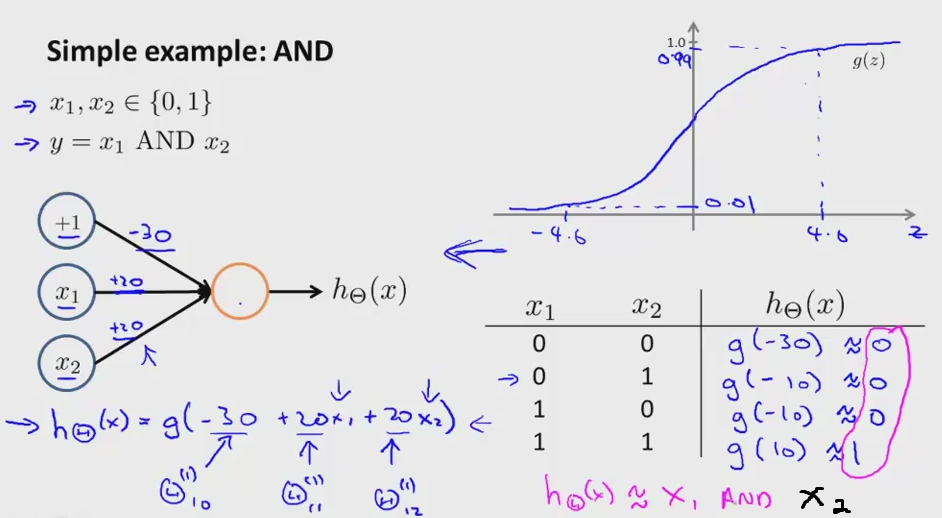
\includegraphics[scale=0.5]{sections/cs229/w5/and_nn.png}
	\end{center}

	\begin{center}
		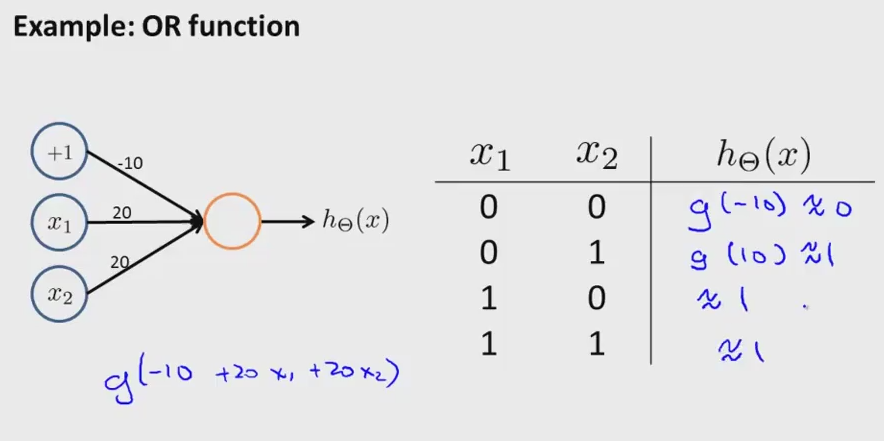
\includegraphics[scale=0.5]{sections/cs229/w5/or_nn.png}
	\end{center}
\end{itemize}

\subsubsection{Examples and Intuitions II}
\begin{itemize}[--]
	\item For models that have non linear boundaries, using a multi-layered network is the best way to approximate the model, for example:
	\begin{center}
		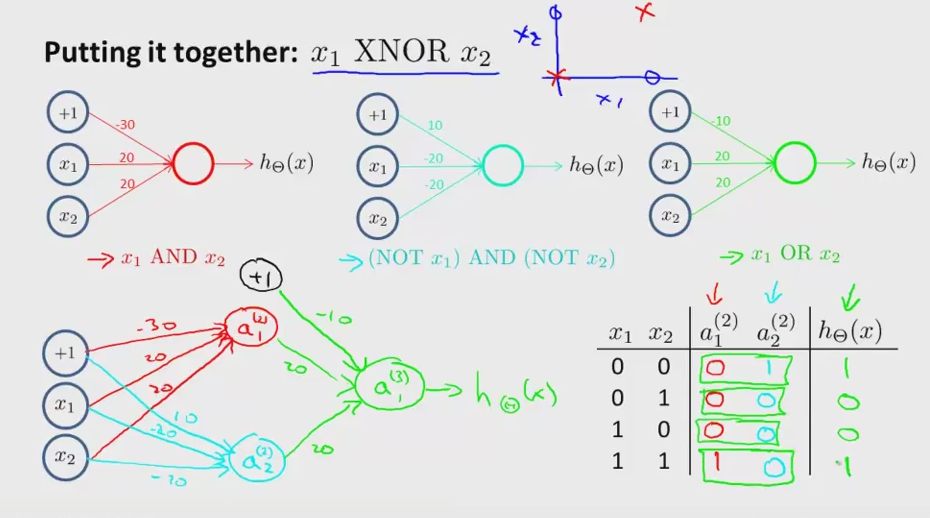
\includegraphics[scale=0.5]{sections/cs229/w5/xnor_nn.png}
	\end{center}

	\item Each layer of the neural network is able to compute even more complex features
	\item The last layer makes the prediction about the correct classification
\end{itemize}

\subsubsection{Multiclass Classification}
\begin{itemize}[--]
	\item Multiclassification is an extension of a one-vs-all 
	\item We want to have the same output units as classes $h(x)\in\mathbb{R}^k$
	\item Each is a classifier for each class, ie. Is it a `1,' is it a `2,' etc..
	\item 
\end{itemize}